\begin{figure}[!h]
\centering
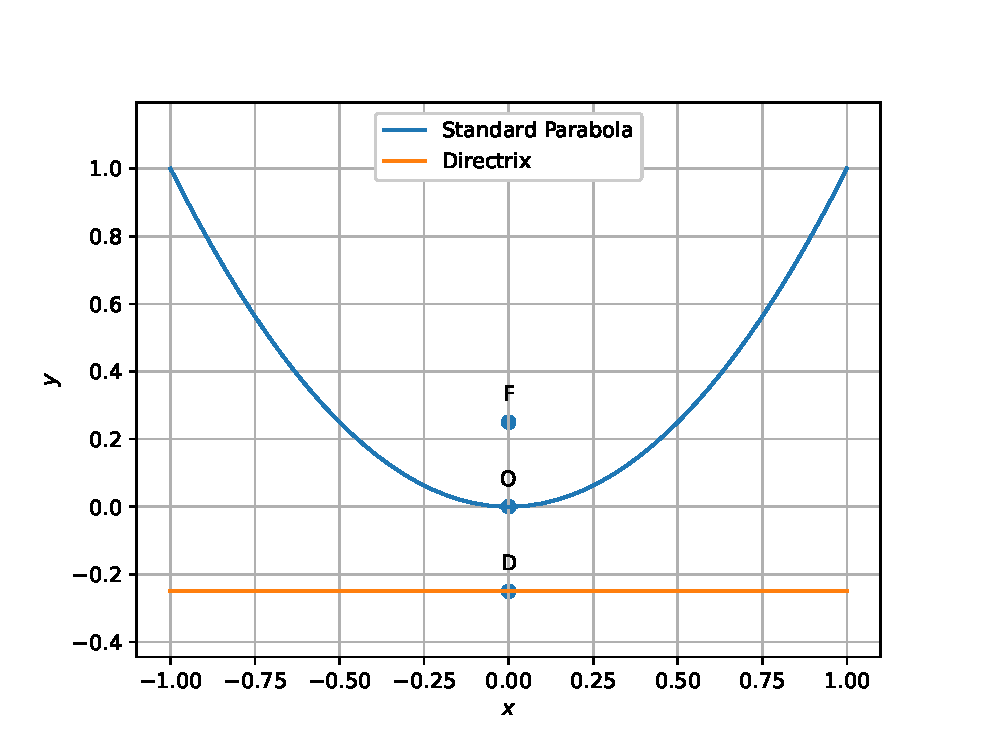
\includegraphics[angle=90,origin=c,width=\columnwidth]{./figs/parabola.eps}
\caption{}
\label{fig:parabola}
\end{figure}
\begin{enumerate}[1.]
\item Show that the line $2y=4x+a$ touches the parabola $y^2=4ax$ and find the coordinates of
the point of contact.
\item Find the point of intersection of the parabolas $y^2=4ax$, $x^2=4ay$ other than the origin, and prove that the tangents
at this point are inclined at an angle $\tan^{-1}\frac{3}{4}$.
\item Find the points in which the line $y=8x-a$ cuts the parabola $y^2=4ax$ and find the point where
the tangents at these points intersect.
\item A line through the vertex $A$ of the parabola $y^2=4ax$ makes an angle of $60\degree$ with
the axis and cuts the curve again in $P$.  Find the equation of the tangent at $P$,
and show that the area of the triangle this tangent makes with the axes is $\frac{4a^2}{3\sqrt{3}}$.
\item Prove that in  Fig. \ref{fig:parabola}
\begin{equation*}
SG=SP
\end{equation*}
\item Prove that $t_1t_2=-1$ is the condition that the chord joining the points $t_1, t_2$ on
a parabola shall pass through the focus.
\item Prove that the tangents drawn to a parabola from a point on the
directrix are at right angles and that their chord of contact passes
through the focus.
\item If in Fig. \ref{fig:parabola} $PS$ cuts the curve again in $Q$, prove that $QA$ passes
through $M$.
\item Through the vertex $A$ of a parabola chords $AP$, $AP$ at right angles
to one another are drawn.  Prove that $PA$ cuts the axis in a fixed point.
\item Find the coordinates of the other point in which the normal at $\brak{at^2,2at}$
meets the parabola $y^2=4ax$; and prove that two normal chords that cut at right angles
divide one another in the ratio $1:3$.
\item Three normals are drawn to a parabola from the point $\brak{h,k}$.  Prove that
the centroid of the triangle formed by their feet is the point $\brak{\frac{2}{3}\brak{h-2a},0}$.
\item Find the equation of the tangent to the parabola $y^2=4ax$ that is parallel
to the normal at $P \brak{at^2,2at}$; and prove that, if this tangent meets the axis in $T$
and $PN$ is the ordinate of $P$ and $A$ is the vertex, then
\begin{equation*}
TA.AN=a^2
\end{equation*}
\item Prove that the circle $x^2+y^2+2gx+2fy+c=0$ cuts the parabola $y^2=4ax$ in four points the sum of
whose ordinates is zero; and conversely that if four ponits on a parabola be
such that the sum of their ordinates is zero then the four points lie on a circle.
\item Prove that the orthocentre of a triangle whose sides all touch a parabola
lies on the directrix.
\item A chord $POQ$ of a parabola $y^2=4ax$ cuts the axis in a fixed point $O$.  $PN$, $QM$ are the ordinates of $P$ and $Q$,
and $A$ is the vertex.  Prove that
\begin{align*}
NP.MQ+4a.AO=0
\end{align*}
\item From a point $P \brak{at_1^2,2at_1}$ on the parabola $y^2=4ax$ two chords $PQ$, $PR$ are drawn normal to the curve at $Q$
and $R$.  Prove that, if $Q$, $R$ are the points $t_2$, $t_3$ on the curve, then $t_2t_3=2$, and the equation
of $QR$ is
\begin{align*}
yt_1+2\brak{x+2a} = 0
\end{align*}
\item Prove that the normals to a parabola at the ends of a chord whose inclination to the axis is $\theta$ meet on the
normal whose inclination is $\tan^{-1}\brak{2\cot\theta}$.
\item Prove that, if two parabolas are on the same side of the same directrix and have their axes in the same line, then they intersect
at a distance from the directrix equal to one-quarter of the sum of their latera recta.

\end{enumerate}
